\documentclass{standalone}
\usepackage{tikz}
\usetikzlibrary{automata,calc,positioning,arrows}

\begin{document}
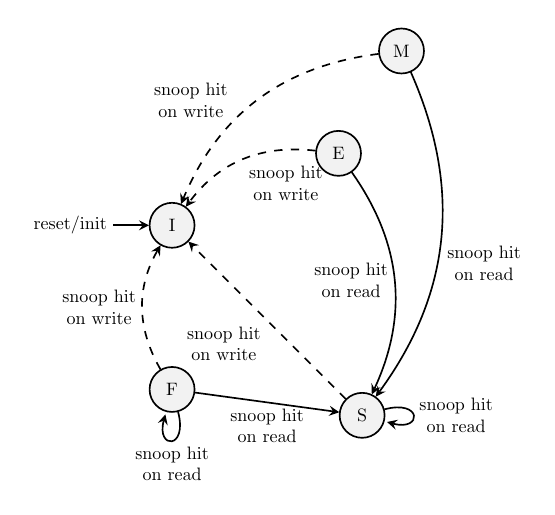
\begin{tikzpicture}[node distance=2.5cm,initial text={reset/init}]
	\tikzstyle{every node}=[scale=0.65]
	\tikzstyle{every state}=[semithick, fill=gray!10]
	\tikzstyle{every edge}=[draw,->,>=stealth,auto,semithick]

	\node[state, initial] (I) {I};
	\node[state,below right= 2cm and 2cm of I] (S) {S};
	\node[state,below= 1.5cm of I] (F) {F};
	\node[state,above right= 0.5cm and 1.7cm of I] (E) {E};
	\node[state,above right= 1.8cm and 2.5cm of I] (M) {M};

	\draw (F)
	edge[loop below] node[align=center] {snoop hit\\on read} (F)
	edge[dashed,bend left] node[align=center] {snoop hit\\on write} (I)
	edge node[align=center,below] {snoop hit\\on read} (S);
	\draw (S)
	edge[loop right] node[align=center] {snoop hit\\on read} (S)
	edge[dashed] node[align=center] {snoop hit\\on write} (I);
	\draw (M)
	edge[bend left] node[align=center] {snoop hit\\on read} (S)
	edge[dashed,bend right] node[align=center,left=0.3cm] {snoop hit\\on write} (I);
	\draw (E)
	edge[bend left] node[align=center,left] {snoop hit\\on read} (S)
	edge[dashed,bend right] node[align=center] {snoop hit\\on write} (I);
\end{tikzpicture}
\end{document}
